%% $RCSfile: proj_report_outline.tex,v $
%% $Revision: 1.3 $
%% $Date: 2016/06/10 03:41:54 $
%% $Author: Mayur Panchal$

\documentclass[11pt
              , a4paper
              , twoside
              , openright
              ]{report}


\usepackage{float} % lets you have non-floating floats

\usepackage{url} % for typesetting urls

%
%  We don't want figures to float so we define
%
\newfloat{fig}{thp}{lof}[chapter]
\floatname{fig}{Figure}

%% These are standard LaTeX definitions for the document
%%                            
\title{Network switching fabric for Gigabit links}
\author{Mayur Panchal}

%% This file can be used for creating a wide range of reports
%%  across various Schools
%%
%% Set up some things, mostly for the front page, for your specific document
%
% Current options are:
% [ecs|msor|sms]          Which school you are in.
%                         (msor option retained for reproducing old data)
% [bschonscomp|mcompsci]  Which degree you are doing
%                          You can also specify any other degree by name
%                          (see below)
% [font|image]            Use a font or an image for the VUW logo
%                          The font option will only work on ECS systems
%
\usepackage[image,ecs]{vuwproject}

% You should specifiy your supervisor here with
%     \supervisor{Firstname Lastname}
% use \supervisors if there is more than one supervisor

\supervisors{Bryan Ng, Robin Dykstra}

% Unless you've used the bschonscomp or mcompsci
%  options above use
%   \otherdegree{OTHER DEGREE OR DIPLOMA NAME}
% here to specify degree

\otherdegree{Bachelor of Engineering with Honours in Electronic and Computer Systems Engineering}

% Comment this out if you want the date printed.
\date{}

\begin{document}

% Make the page numbering roman, until after the contents, etc.
\frontmatter

%%%%%%%%%%%%%%%%%%%%%%%%%%%%%%%%%%%%%%%%%%%%%%%%%%%%%%%

%%%%%%%%%%%%%%%%%%%%%%%%%%%%%%%%%%%%%%%%%%%%%%%%%%%%%%%

\begin{abstract}

A short description of the project goes here.

\end{abstract}

%%%%%%%%%%%%%%%%%%%%%%%%%%%%%%%%%%%%%%%%%%%%%%%%%%%%%%%

\maketitle

\chapter*{Acknowledgments}\label{C:ack} 
Any acknowledgments should go 
in here, between the title page and the table of contents.  The 
acknowledgments do not form a proper chapter, and so don't get a 
number or appear in the table of contents.

\tableofcontents

% we want a list of the figures we defined
\listof{fig}{Figures}

%%%%%%%%%%%%%%%%%%%%%%%%%%%%%%%%%%%%%%%%%%%%%%%%%%%%%%%

\mainmatter

%%%%%%%%%%%%%%%%%%%%%%%%%%%%%%%%%%%%%%%%%%%%%%%%%%%%%%%

% individual chapters included here
\chapter{Introduction}\label{C:intro}

\par Fast internet connections are becoming more and more desired as high bandwidth media consumption and internet 
based services grow in popularity. Speed of an internet connection can be separated into two distinct metrics, 
latency and bandwidth. Latency is the time taken for information to travel from one place to another and the delay 
introduced by the device itself, while bandwidth is the amount of information that can flow reliably from end to end.
When a user is accessing a website, such as Facebook, their requests traverse multiple network devices (physical 
hardware) to reach that website's servers. Throughout this travel, each network device introduces some latency, as 
there is processing time required to send information to the right destination. Although this delay is very small, 
over the course of multiple hops it can become significant. Measuring this small latency with current solutions is
convoluted and without the right systems, can be unreliable. By measuring this latency, we can enable research to
reduce latency to create a faster internet.

\section{Problem}

\par There has been research dedicated to reducing latency. Some ways to reduce this latency include making “smart” network routers \cite{smartrouters} and low latency wireless systems \cite{5g}. 
This research is reaching the point where network traffic can have latency as little as 1ms \cite{lessthan1ms} or below.
To advance further, new tools need to have the capability of measuring this latency.

\par Existing hardware solutions to measuring latency are capable of measuring less than 1 ms but require some 
additional training in the software suite provided with the hardware \cite{dagfeatures}. Additional processes attached
to hardware based methods can require dedicated computers for the measurement and analysis of networks. This means 
that each researcher would require an understanding of the software suite accompanied with a dedicated computer 
all setup for specific tests to be run. Each different test would require reconfiguring of both hardware and software.
This drives the cost of using the device up, in terms of both time and money.

\par Current software solutions can measure latency in ethernet network traffic down to a resolution of
milliseconds and sometimes microseconds \cite{pingisbad}. There are no software solutions that can measure
latency in the order of nanoseconds reliably \cite{timeinlinux}. Measuring the latency in nanoseconds is needed as
network switches have very low latency and the time between ingress and egress can range from
microseconds to nanoseconds. If it could be measured accurately, then analysis could be performed
on network traffic through network switches to research new ways to reduce latency.

\par Existing methods to measure latency within microseconds and nanoseconds require monolithic devices which need 
setting up and installing device drivers, proprietary software, or even a replacement of existing hardware systems.
Once setup, these devices often require data conversion of results to be compatible with data analysis methods and 
evaluation programs. Occasionally these programs are embedded within in manufacturers software, but the user is 
limited to what the manufacturer has chosen as relevant outputs for the user. These can be useful most of the time, 
but occassionally the user would need to export the data to another data analysis tool they are familiar with for 
futher processing. This inflexibility is prominent in many high end network performance analysis tools, causing 
delays in retrieving test results for evaluation.

\par A reduction in network latency would be a huge boon to future technologies. For example, less
latency in video streaming can enable doctors from remote locations to perform surgery with
minimal lag between actions and responses \cite{remotesurgery}. The stock market is another example of improvement with
this technology, as less latency ensures that stock market trade deals can be completed faster.

\begin{quote}
    \centering
    ``We are running through the United States with dynamite and rock saws, so that an algorithm can
    run three microseconds faster.`` \em --- Kevin Slavin, How Algorithms shape our world \cite{tedTalkAlgorithms}
\end{quote} 

\par Many improvements made at a nanosecond scale can add up to microseconds or even milliseconds of latency
reduction. Improvements cannot be done without knowing how much this can improve by without the tools to measure it.

\par A software based approach has the limitation that the timing functions must be processed by a
Central Processing Unit (CPU) \cite{CPUtiming}. This means the counters for timing functions could be offset from the true value. Higher
resolution latency measurements can be achieved through a hardware implementation of a packet
timer. This circumvents the limitations of a software based approach.

\section{Solution}

Latency occurs the instant that a network packet is sent from a computer. The processing times for the network packet
to flow through the networking stack in the operating system can be considered a constant unavoidable delay which is
not in the scope of this project.

Because the nature of when the latency occurs, it would be best measured by considering the raw electronic signals 
from the ethernet port on the device to ensure there is no operating system lag. To achieve this, microcontrollers, 
discrete logic gates and a Field Programmable Gate Array could be implemented. A microcontroller could be used but 
then the same issues arise, that a CPU clocking through instructions would deviate the true timing counter value. 
Another approach would be to use discrete logic gates to measure the timing accurately, but this will become 
complicated very rapidly, and propagation delays through discrete devices would reduce the accuracy. Hence the 
preferred choice is to implement the packet latency measurement unit on a Field Programmable Gate Array (FPGA). More 
information about FPGA’s is in the Background section of the report. This way complex digital designs can be 
simplified down to a simple set of blocks, and there is no overhead that a processor would introduce. The drawback 
to using an FPGA is that the learning curve to developing on the platform is quite steep, and also communication 
with existing systems is difficult and is usually aided by the use of a microcontroller (such as an ARM or x86 based 
co-processor)

\par This report will focus on the work done so far in implementing a FPGA based packet latency timing
device. This project is limited to Ethernet based networks as they are most widely used \cite{etherneteverywhere}.

\chapter{Background}\label{C:back}

\section{Network packet}

\par Communication between computers is established through the means of physical connections and protcols overlaying on top of this. 
A widespread communication protocol is to break down each point of communication into discrete pieces called network packets.
These network packets contain many layers (Figure: \ref{fig:OSIModel}) of communication information.
Communication layers can be broken down into a few independent layers which hold specific purposes. 
Each layer contains information which can aid with transporting the information to the correct computer securely.
As each layer is independent, each higher layer does not affect the forthcoming layers.
High layers of the model are for purposes such as reliability of data and the data itself in the packet.
For the purposes of this project, an explanation of only the first three layers of the Open Systems Interconnection (OSI) model is concerned.

\begin{figure}[H]
    \begin{center}
        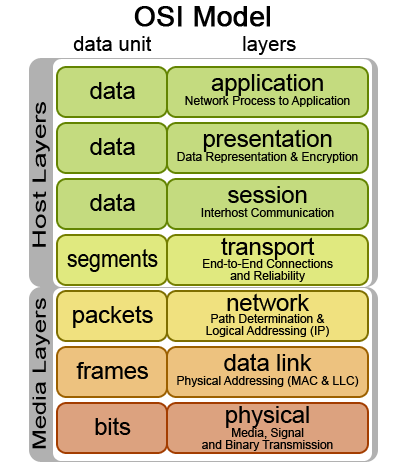
\includegraphics[width=5cm,height=5cm,keepaspectratio]{Images/OSIModel.png}
        \caption{OSI Model}
        \label{fig:OSIModel}
    \end{center}
\end{figure}

\subsection{Layer 1: Physical}

\par The physical layer is specifying the electrical and physical medium that is used to transport individual bits from one computer to another.
Two or more computers can be connected through many different physical mediums such as copper wiring and light fibers. 
Each medium has specific pros and cons, from implementation costs to throughtput capabilities.
The physical layer is responsible for transmitting and receiveing unstructured data.
Communication can be either Simplex, Half Duplex or Full Duplex.
The network topology is defined by how the physical layer is configured.
An example of a phyiscal medium is a copper medium is used to link two devices together.
This project will be investigating the latency present in a Gigabit Ethernet system, using copper based medium.

\subsection{Layer 2: Data link}

Data link layer is responsible for node-to-node data communication. 
It links from one device to another, determing the connection status of two physically connected devices.
A feature of this layer, is the ability to detect and correct errors created at the physical layer.
The IEEE Standard 802 \cite{IEEE802} details how this layer is split into two sub layers, Media Access Control (MAC), and Logical Link Control (LLC).
This project will cover networking switches which distinguish different destination devices by their unique MAC addresses.

\subsection{Layer 3: Network}

Network layer provides functionality when sending data across a network.
End-to-end communication is aided by assigning each node in the network an address, which it identifies itself with.
This allows data to be passed through intermediate nodes, which would continue to traverse until the target node has been reached.
This project will not be including this layer, or any others higher than this, as the latency measurements involved are short, single node-to-node distances.

\section{Network Latency}

\subsection{Connection Time}

\subsection{Round Trip Time}

\section{Current Timing Solutions}

Timing of network packets can currently done through very expensive and bulky devices. 
For this reason, there are many software implementations that allow high speed packet processing.
The following software implementations have some restrictions on what hardware they can run on.
The precision to measure the latency of packets is unknown and needs to be investigated.
This project is to combine the flexibility of software and hardware to create a packet latency measurement utility.

\subsection{Data Plane Development Kit (DPDK)}

Data Plane Development Kit (DPDK) is a set of C libraries to allow for rapid processing of network packets.
It utilizes a few low level Application Programming Interfaces (APIs) to minimize the overhead of using a specific architecture computer.
Reducing this overhead of the CPU reduces the amount of latecy present in the act of measuring the time between packets itself.
This is a very good software solution to what is currently on the market, but one caveat to using this technology is that only specific hardware can be used.
The Network Interface Card (NIC) on the computer has to be compatible with the software.

\subsection{PF\textunderscore RING}

PF\textunderscore RING by ntop\texttrademark is a software solution for rapid network packet processing.
It is a network socket technology which improves the speed at which packets are captured by the processor.
Faster packet processing ensures that the time stamp placed on an ingress packet is accurate as it can be.
This is a software solution which could potentially work well, but is limited by the software latency of needing to be processed by a processor.
The NIC on the computer does not have to be a specific model, meaning this is a much more flexible solution.

\section{Measurement Techniques}

\subsection{Cut-Through}

\subsection{Store-and-Forward}

\section{Field Programmable Gate Array}

\subsection{Reconfigurable Macro Cells}

\subsection{FPGA vs Microcontroller}

%% $RCSfile: using.tex,v $
%% $Revision: 1.1 $
%% $Date: 2010/04/23 01:57:05 $
%% $Author: kevin $
%%
\chapter{Using this document and the \texttt{vuwproject} style}\label{C:us}

If you are writing an MSc or PhD thesis you should \emph{not} be using this style. Instead use \verb=vuwthesis=, which is based on the book style, and conforms to the VUW thesis rules. The thesis style is rather different from the project report style. 

This document is formatted using a local (to ECS and MSOR at VUW) style file. When you write your project report you should be very careful when changing the beginning. The document class settings should read:

\begin{verbatim}
\documentclass[11pt
              , a4paper
              , twoside
              , openright
              ]{report}
\end{verbatim}
The options to the document class specify that:
\begin{itemize}
\item 11pt font is to be used for the main body text,
\item  we will print on A4 paper, 
\item we will use duplex (two-sided) printing,
\item we want chapters to start on a right-hand page. 
\end{itemize}

The opitons you supply to the  \texttt{vuwproject} style will depend upon
what you are using the style for.

\subsection{Specifying the details}
The \texttt{vuwproject} style sets up the front page properly, and provides various commands allowing you to specify the author, title, supervisor or supervisors, the school from which the report is being submitted and the degree that the report is being submitted for. The style has deliberately been designed to do as little as possible. This means that your document can easily be re-formatted as a technical report, or for submission to a conference or journal by using the appropriate style.

It is also possible to use the style to easily produce documents on a
stand-alone computer where your \LaTeX installtion might not have all
of the  files and fonts available to machines within ECS or MSOR.

Most of the options to the \texttt{vuwproject} style are currently a simple
choice and there's a default that will make it obvious if you do not make
a choice.

Use one of the following options to use fonts available on ECS/MSOR machines
or to use images that imitate them (assumes you have copies of the images)
\begin{itemize}
\item \verb+font+
\item \verb+image+
\end{itemize}

Use one of the following options to set the school,
\begin{itemize}
\item \verb+ecs+
\item \verb+msor+
\end{itemize}

Use one of the following options to choose a pre-defined degree,
\begin{itemize}
\item \verb+bschonscomp+
\item \verb+mcompsci+
\end{itemize}

or use this command to use an explicit degree or diploma name
\begin{itemize}
\item \verb+\otherdegree{DEGREE OR DIPLOMA NAME}+
\end{itemize}

So, for example, to submit a report for the Master of Comp Sci degree, which
the style knows about, from within ECS, using the images, you'ld ensure the
 \texttt{vuwproject} line options looked like:

\begin{verbatim}
\usepackage[image,ecs,mcompsci]{vuwproject}
\end{verbatim}

whereas for a degree from within MSOR, when creating the final version on
an ECS or MSOR machine where you have access to the fonts, you would use
these options

\begin{verbatim}
\usepackage[font,msor]{vuwproject}
\end{verbatim}


and add the other degree's name using this command 

\begin{verbatim}
\otherdegree{DEGREE OR DIPLOMA NAME}
\end{verbatim}

To specify the supervisor or supervisors use either of the following commands in the preamble.
\begin{itemize}
\item \verb+\supervisor{The Supervisor}+
\item \verb+\supervisors{Super 1 and Super 2}+
\end{itemize}

If you fail to set any degree or supervisor, or the school, then the front page will report this.

The \texttt{vuwproject} style also sets the default font to be Palatino, using the \texttt{mathpazo} package. Palatino is one of VUW's `offical' fonts, and is the font used for the heading on the front page. The \texttt{mathpazo} package also typesets maths in a style which suits Palatino. 

\section{Copying the style}
If you want to write your project report away from VUW you will need to make your own copy of the \texttt{vuwproject} style.

You can find out where the original lives by reading the messages that \LaTeX\ prints when it is run.

Alternatively, you can down load a copy of the  \texttt{vuwproject} style from
the ECS webpages.

Any changes made to your own copy of the \texttt{vuwproject} style will not be reflected in the original, and \textit{vice versa}. Hence it makes sense to leave this as it is, and use a local style file for your own definitions.   

\chapter{Some \LaTeX\ hints and tips}\label{C:ex}
\LaTeX\ is a very good tool for producing well-structured documents 
carefully. It is very bad tool for banging things together in a rush 
and panic. 

\section{Floats}
One perennial problem with \LaTeX\ is its treatment of 
\emph{floats}.  Suppose you have a figure or table which you want to 
include in your document. Where should it go? Traditional typesetting 
practice is to put these in some convenient place, such as the top or 
bottom of the current or next page, or at the end of the section or 
chapter.  \LaTeX\ adopts a similar strategy, and allows floats to 
``float'' away from where they were defined. You can give a hint 
about where you want the figure, but \LaTeX\ may move it. Sometimes 
this is fine but sometimes you may want to have more control and 
insist that a float goes \emph{here}. Anselm Lingau's 
\textsf{float} package gives you this flexibility. For example, the following figure is an example of a non-floating float:

\begin{fig}[H]
\begin{center}
\begin{tabular}{l|lll}
$\delta$ & $\mathit{a}$ & $\mathit{b}$ & $\Lambda$ \\ \hline 
$S_{1}$  & $\{\}$       & $\{\}$      & $\{S_{2}, S_{5}, S_{10}\}$\\
$S_{2}$  & $\{S_{3}\}$  & $\{\}$      & $\{\}$\\
$S_{3}$  & $\{S_{4}\}$  & $\{\}$      & $\{\}$\\
$S_{4}$  & $\{S_{3}\}$  & $\{\}$      & $\{\}$\\
$S_{5}$  & $\{\}$       & $\{S_{6}\}$ & $\{\}$\\
$S_{6}$  & $\{\}$       & $\{S_{7}\}$ & $\{S_{8}\}$\\
$S_{7}$  & $\{S_{6}\}$  & $\{\}$      & $\{\}$\\
$S_{8}$  & $\{S_{9}\}$  & $\{\}$      & $\{\}$\\
$S_{9}$  & $\{\}$       & $\{S_{8}\}$ & $\{\}$\\
$S_{10}$ & $\{S_{11}\}$ & $\{\}$      & $\{\}$\\
$S_{11}$ & $\{\}$       & $\{S_{10}\}$& $\{\}$\\ 
\end{tabular}
\caption{The transition function of an NFA with $\Lambda$  transitions}

\end{center}
\end{fig}

On the other hand, Figure \ref{Fig:two} is a floating float. 



\begin{fig}[tbh]
\begin{center}
\begin{tabular}{l|ll}
$\delta''$ & $\mathit{a}$ & $\mathit{b}$ \\ \hline 
$T_{1}$  & $T_{2}$ & $T_{3}$\\ 
$T_{2}$  & $T_{4}$ & $T_{5}$\\ 
$T_{3}$  & $T_{6}$ & $T_{7}$\\ 
$T_{4}$  & $T_{8}$ & \\
$T_{5}$  & $T_{10}$ & \\
$T_{6}$  &  & $T_{11}$\\ 
$T_{7}$  & $T_{3}$ & \\
$T_{8}$  & $T_{4}$ & \\
$T_{10}$  &  & $T_{5}$\\ 
$T_{11}$  & $T_{6}$ & 
\end{tabular}
\caption{The transition function of an FA to accept 
the same language.}
\label{Fig:two}
\end{center}
\end{fig}

You can define different types of new floats, and you can have tables 
of them in the contents pages.


\section{URL's}
Use \verb=\url= from the \textsf{url} package to typeset URL's. Just 
using \verb+\texttt+ or \verb+\tt+ does not work:

\begin{itemize}
\item \verb+\texttt{http://www.mcs.vuw.ac.nz/~neil/}+
\item \verb+\url{http://www.mcs.vuw.ac.nz/~neil/}+
\end{itemize}

Give:
\begin{itemize}
\item \texttt{http://www.mcs.vuw.ac.nz/~neil/}
\item \url{http://www.mcs.vuw.ac.nz/~neil/}
\end{itemize}
If you use the \textsf{hyperref} package then you can produce PDF 
files with clickable hyperlinks using \verb=\url=.

\section{Graphics and \LaTeX}
\LaTeX\ offers rather poor support for the inclusion of graphics. 
There are lots of ways to include pictorial material in \LaTeX, all 
of which are deficient in some way or other. Look at \cite{GRM97GC} for a 
description of them. If your document does need to have pictures in it 
it is worth thinking about what is needed \emph{before} you generate 
the pictures.

\section{The bibliography}

You should build up your bibliography as you go along.  Trying to get 
the details of the bibliography correct at the end of the project is 
hard work. Make sure that you record all the relevant details. Beware 
that material on the internet is likely to change very rapidly. If you 
are going to include material which is only available on the internet, 
then you should probably include in the reference the date on which 
you obtained the document.

\section{Run \LaTeX, run}

\LaTeX\ builds up information about your document for the table of 
contents, references and so on at each run. This means that, for 
example, the table 
of contents is really the table of contents of the previous 
compilation. You may need to run \LaTeX\ two or three times to let it 
catch up with itself. If you have cross references within your 
bibliography (for example two papers from the same collection, such 
as \cite{Dum93a,Dum93b}) you may need to run 
BibTeX more than once. 

It is also possible that the table of contents file has garbage in 
it, and will prevent the document from being compiled. This may 
happen if you have had to abort compilation, due to a bug in the 
source file. If this is the case then removing the \texttt{.toc} file 
will usually solve the problem. You will have to fix the original 
bug, of course.


\section{Find out more by\ldots}
You can find out more by:
\begin{itemize}
\item reading any one of a number of books, such as \cite{GMS94,Lam94}. The 
VUW library has copies of these;
\item visiting  the Comprehensive \TeX\ Archive Network (CTAN) at 
\url{www.ctan.org};
\item typing \texttt{latex} into Google.
\end{itemize}

It is \emph{highly unlikely} that you are the first person who ever 
wanted to do what you want to do with \LaTeX. Therefore it is likely 
that someone has already solved your problem: the real key to using  
\LaTeX\ well is to make effective use of what other people have done.

\section{Summary}
In this chapter we explained some things about \LaTeX.
\chapter{Future Work and Conclusion}\label{C:conc}

As the device is a minimum viable product, there are many improvements that can be made to make the device more 
reliable and flexible. 

\section{ID Packets}

Currently the device has a standard packet format which is hard coded into the FPGA fabric, to produce network 
packets. The idea of producing packets with increasing IDs can ensure that tests can be run in parallel and would 
not interfere with each other. This is the hypothesized reason for the short latencies produced during testing. This 
would help ensure that each test is independent and could also remove the problem of very short outliers in the 
results.

\section{Connect to the Internet for added Flexibility}

The device made has a spare ethernet port to connect to an internet connected network. This would allow the device 
results to be published to cloud based information aggregators such as AWS Kinesis.

\section{Remote Connectivity}

Connecting the device to a network, would allow an operator to connect to the device remotely and run tests without 
being physically present with the device. This would be advantageous in a datacentre setting, as locations of 
servers are commonly a harsh environment for humans to be in. To allow the remote connection to the device, a Linux 
image would need to be created with a Linux program to run the tests. 

\section{Custom Hardware}

The Zedboard and Ethernet FMC card both contain extra hardware which is not utilized in this project. A custom PCB 
with the FPGA would be able to significantly reduce the cost of entry to this platform by mass manufacturing a PCB 
with only the required components on board.

\section{Conclusion}

The device is currently a minimum viable product. The device can provide high resolution and reliable timings in a 
flexible format.  This is useful for new research being done with high speed communications as the need for faster 
data transfer grows and the measurement of smaller and smaller latencies is becoming more of an issue. This is 
currently solved by using one of the many hardware device platforms that are available, but these do not offer 
flexible way of obtaining results and require training in using the device.  Software platforms provide the 
flexibility that hardware systems do not provide, but produce inconsistent and unreliable results.

As shown by this device, hardware platforms can be both flexible and provide reliable testing results. This device 
fills a gap in the market where no proprietary software is needed to accompany the device for network packet analysis. 



%%%%%%%%%%%%%%%%%%%%%%%%%%%%%%%%%%%%%%%%%%%%%%%%%%%%%%%

\backmatter

%%%%%%%%%%%%%%%%%%%%%%%%%%%%%%%%%%%%%%%%%%%%%%%%%%%%%%%


%\bibliographystyle{ieeetr}
\bibliographystyle{ieeetr}
\bibliography{sample}


\end{document}
